%%%%%%%%%%%%%%%%%%%%%%%%%%%%%%%%%%%%%%%%%%%%%%%%%%%%%%%%%%%%%%%%%%%%%%%%%%%%%%%%
% Preámbulo                                                                    %
%%%%%%%%%%%%%%%%%%%%%%%%%%%%%%%%%%%%%%%%%%%%%%%%%%%%%%%%%%%%%%%%%%%%%%%%%%%%%%%%
\documentclass[11pt,a4paper,titlepage,oneside]{report}

%%% RELACIÓN DE VARIABLES A PERSONALIZAR %%%
%\def\lingua{gal}
\def\lingua{esp} % descomenta esta liña se redactarás a memoria en español
%\def\lingua{eng} % descomenta esta liña se redactarás a memoria en inglés
\def\nomeA{Óscar Olveira Miniño}
\def\nomeB{Alejandro Javier Herrero Arango}                     % substitúe aquí o teu nome
%\def\nomedirectorB{Outro Nome Completo}             % duplica esta liña máis veces se o precisas, cambiando
                                                     % a letra final (A, B, C, D...): úsanse na portada.tex
\def\titulo{Práctica 1: DiffServ en INET} % substitúe aquí o título do teu TFG
%\def\titulacion{gced}                               % descomenta esta liña e comenta a seguinte se es estudante do GCED
\def\titulacion{gei}
%\def\mencion{COMPUTACIÓN}                           % descomenta a mención que che corresponda se es estudante do GEI
%\def\mencion{ENXEÑARÍA DO SOFTWARE}
%\def\mencion{ENXEÑARÍA DE COMPUTADORES}
%\def\mencion{SISTEMAS DE INFORMACIÓN}
\def\mencion{TECNOLOXÍAS DA INFORMACIÓN}

%\def\renomearcadros{si} % descomenta esta liña se redactas a memoria en español e prefires que
                         % os "cuadros" e o "índice de cuadros" se renomeen
                         % a "tablas" e "índice de tablas" respectivamente

\usepackage{estilo_tfg}
\usepackage{tcolorbox}
% Lista de paquetes potencialmente interesantes (uso baixo demanda)

% \usepackage{alltt}       % proporciona o entorno alltt, semellante a verbatim pero que respecta comandos
% \usepackage{enumitem}    % permite personalizar os entornos de lista
% \usepackage{eurofont}    % proporciona o comando \euro
% \usepackage{float}       % permite máis opcións para controlar obxectos flotantes (táboas, figuras)
% \usepackage{hhline}      % permite personalizar as liñas horizontais en arrays e táboas
  \usepackage{longtable}   % permite construir táboas que ocupan máis dunha páxina
% \usepackage{lscape}      % permite colocar partes do documento en orientación apaisada
% \usepackage{moreverb}    % permite personalizar o entorno verbatim
% \usepackage{multirow}    % permite crear celdas que ocupan varias filas da mesma táboa
% \usepackage{pdfpages}    % permite insertar ficheiros en PDF no documento
% \usepackage{rotating}    % permite diferentes tipos de rotacións para figuras e táboas
% \usepackage{subcaption}  % permite a inclusión de varias subfiguras nunha figura
% \usepackage{tabu}        % permite táboas flexibles
% \usepackage{tabularx}    % permite táboas con columnas de anchura determinada

%%%%%%%%%%%%%%%%%%%%%%%%%%%%%%%%%%%%%%%%%%%%%%%%%%%%%%%%%%%%%%%%%%%%%%%%%%%%%%%%
% Corpo                                                                        %
%%%%%%%%%%%%%%%%%%%%%%%%%%%%%%%%%%%%%%%%%%%%%%%%%%%%%%%%%%%%%%%%%%%%%%%%%%%%%%%%

\begin{document}

 %%%%%%%%%%%%%%%%%%%%%%%%%%%%%%%%%%%%%%%%
 % Preliminares do documento            %
 %%%%%%%%%%%%%%%%%%%%%%%%%%%%%%%%%%%%%%%%

 \begin{titlepage}
  
  \hspace*{128pt}
  \textcolor{udcpink}{{\fontencoding{T1}\fontfamily{phv}\selectfont Facultade de Informática}}\\[-32pt]

  \begin{center}
    
\includegraphics[scale=0.3]{imaxes/udc}\\[25pt]

    {\large TRABALLO FIN DE GRAO \\
            \nometitulacion \\
            \nomemencion } \\[10pt]

    \carimbo \\[25pt]

    \begin{huge}
      \begin{spacing}{1.3}
        \bfseries \titulo
      \end{spacing}
    \end{huge}
  \end{center}
  
  \vfill
  
  \begin{flushright}
    {\large
    \begin{tabular}{ll}
      {\bf Estudante 1:}& \nomeA\\
      {\bf Estudante 2:}& \nomeB
%                      & \nomedirectorB \\ % duplica esta liña máis veces se o precisas, cambiando
                                           % a letra final (A, B, C, D...); define eses nomes no memoria_tfg.tex
    \end{tabular}}
  \end{flushright}
  \rightline{A Coruña, \datasimple.}
\end{titlepage}

 %\dedicatoria{Dedicatoria} % escribe neste comando o teu texto de dedicatoria
 %\paxinaenbranco
 %\begin{agradecementos}
 %\blindtext                % substitúe este comando polo teu texto de agradecementos
 %\end{agradecementos}
 %%%%%%%%%%%%%%%%%%%%%%%%%%%%%%%%%%%%%%%%%%%%%%%%%%%%%%%%%%%%%%%%%%%%%%%%%%%%%%%%%

\pagestyle{empty}
\begin{abstract}
  \blindtext % substitúe este comando polo resumo do teu TFG
             % na lingua principal do documento (tipicamente: galego)

  \vspace*{25pt}
  \begin{segundoresumo}
    \blindtext % substitúe este comando polo resumo do teu TFG
               % na lingua secundaria do documento (tipicamente: inglés)
  \end{segundoresumo}
\vspace*{25pt}
\begin{multicols}{2}
\begin{description}
\item [\palabraschaveprincipal:] \mbox{} \\[-20pt]
  \blindlist{itemize}[7] % substitúe este comando por un itemize
                         % que relacione as palabras chave
                         % que mellor identifiquen o teu TFG
                         % no idioma principal da memoria (tipicamente: galego)
\end{description}
\begin{description}
\item [\palabraschavesecundaria:] \mbox{} \\[-20pt]
  \blindlist{itemize}[7] % substitúe este comando por un itemize
                         % que relacione as palabras chave
                         % que mellor identifiquen o teu TFG
                         % no idioma secundario da memoria (tipicamente: inglés)
\end{description}
\end{multicols}

\end{abstract}
\pagestyle{fancy}

%%%%%%%%%%%%%%%%%%%%%%%%%%%%%%%%%%%%%%%%%%%%%%%%%%%%%%%%%%%%%%%%%%%%%%%%%%%%%%%%


 \pagenumbering{roman}
 \setcounter{page}{1}
 \bstctlcite{IEEEexample:BSTcontrol}

 \tableofcontents
 \listoffigures
 %\listoftables
 \clearpage
 
 \pagenumbering{arabic}
 \setcounter{page}{1}

 %%%%%%%%%%%%%%%%%%%%%%%%%%%%%%%%%%%%%%%%
 % Capítulos                            %
 %%%%%%%%%%%%%%%%%%%%%%%%%%%%%%%%%%%%%%%%

 \chapter{Router sin QoS}
\label{chap:sinqos}

\section{Longitud de cola del router}

\subsection{Para el caso en el que se están transmitiendo tanto el flujo VoIP como los dos flujos UDP, calcula:}

\renewcommand{\theenumi}{\alph{enumi}}
\begin{enumerate}
    \item Tasa de entrada [pkt/s] a la cola.

\[
\label{eq:sinqos_tasa_entrada}
R_{in} = R_{VoIP} + 2 \cdot R_{UDP} = \frac{1~\mathrm{pkts}}{20~\text{ms}} + 2 \cdot \left(\frac{1 ~ \text{pkts} }{80 ~ \text{ms} }\right) = \frac{1~\mathrm{pkt}}{0,02~\text{s}} + \frac{2~\mathrm{pkt}}{0,08~\text{s}} = 50 ~ \text{pkt/s} + 25 ~ \text{pkt/s} = 75 ~ \text{pkt/s}
\]

    \item Proporción de paquetes de cada tipo en la cola.

    En VoIp: \[ \frac{R_{VoIP}}{R_{in}} = \frac{50~\text{pkts/s}}{75~\text{pkts/s}} = \frac{2~\text{pkts/s}}{3~\text{pkts/s}}  \approx 66,66\%\]

    En UDP: \[ \frac{R_{VoIP}}{R_{in}} = \frac{25~\text{pkts/s}}{75~\text{pkts/s}} = \frac{1~\text{pkts/s}}{3~\text{pkt/s}} \approx 33,33\% \] 
            (ambos transmisores UDP, cada uno tiene una proporción de \( 16,67\% \)).

    \item Tasa de salida [pkt/s] de la cola, asumiendo que la cabecera del protocolo PPP tiene 7B.
 
    Como está la cabecera PPP de 7B, los paquetes VoIP tendría una cabecera total de 199B y los paquetes UDP una cabecera de 1000B.

    \begin{eqnarray}
        \label{eq:senqos_tasa_salida}
        128~\text{kb/s} \cdot \frac{1000~\text{b}}{1~\text{kb}} \cdot \frac{1~\text{B}}{8~\text{b}} = 16000~\text{B/s} \\
        R_{out} = \frac{16000~\text{B/s}}{ \frac{2}{3} \cdot  199~\text{B/pkts} + \frac{1}{3} \cdot 1000~\text{B/pkts}} = 34,33~\text{pkts/s}
    \end{eqnarray}


    \item ¿Cuánto tarda en llenarse la cola?
    
    Como se ve en la gráfica tamaño de la cola sin QoS, tiene un tamaño de 100pkts:

    \[
    \label{eq:sinqos_tiempo_llenado}
      T_{fill} = \frac{L}{R_{fill}} = \frac{L}{R_{in} - R_{out}} \frac{100~\text{pkts}}{75~\text{pkt/s} - 34,33~\text{pkts/s}} = 2,46~\text{s}
    \]


\end{enumerate}

\subsection{¿Cuál es la tasa de entrada [pkt/s] y la tasa de salida [pkt/s] justo en el momento en que deja de
transmitirse el flujo VoIP? ¿Qué consecuencia tienen estas tasas sobre la cola?}
La tasa de entrada al dejar de transmitir los paquetes de VoIP, solamente se transmiten los paquetes UDP, entonces en la ecuación \ref{eq:sinqos_tasa_entrada},
solo tendríamos en cuenta la tasa de los paquetes UDP, quedando en:
    
\[
  R_{in} = R_{UDP1} + R_{UDP2} = \frac{1~\mathrm{pkts}}{80~\mathrm{ms}} + \frac{1~\mathrm{pkts}}{80~\mathrm{ms}} = 12,5~\mathrm{pkts/s} + 12,5~\mathrm{pkts/s} = 25~\mathrm{pkts/s}
\]

La tasa de salida, aunque dejemos de transmitir paquetes VoIP, según la ecuación \ref{eq:sinqos_tiempo_llenado}, la cola se llena a los 2,46 segundos
por lo que después de 60s (cuando se deja de transmitir VoIP), la cola seguirá llena entonces la tasa de salida sigue siendo igual hasta que 
se empiece a vaciar.

La consecuencia de tener estas nuevas tasas es que la cola se va a vaciar, ya que: \[R_{in} < R_{out}\]
Una vez pasado un tiempo, la tasa de salida va a ser:

\[
  128~\text{kb/s} \cdot \frac{1000~\text{b}}{1~\text{kb}} \cdot \frac{1~\text{B}}{8~\text{b}} = 16000~\text{B/s} \\
  R_{out} = \frac{16000~\text{B/s}}{1000~\text{B/pkts}} = 16~\text{pkts/s}
\]

En ese momento, al ser la tasa de entrada más grande que la tasa de salida, se va a volver a llenar la cola. Este problema se puede observar
en la gráfica \ref{fig:sinqos_tam}.

\begin{figure}[!ht]
    \centering
    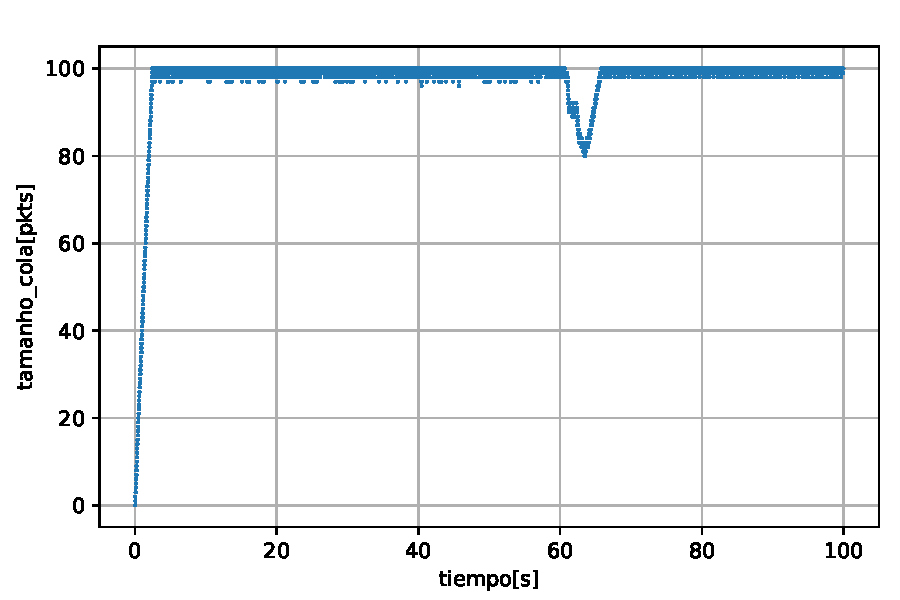
\includegraphics{graficas/sinQoS/tamanho_cola_sinQoS.pdf}
    \caption{Longitud de la cola del router sin QoS}
    \label{fig:sinqos_tam}
\end{figure}

\subsection{Para el caso en el que ya solo se están transmitiendo los dos flujos UDP y la cola solo contiene paquetes
UDP, calcula la tasa de entrada [pkt/s] y tasa de salida [pkt/s]}

Estas dos tasas ya se han calculado en el siguiente apartado. Por lo tanto quedaría que:

\[
  R_{in} = 25~\mathrm{pkts/s}
\]

\[
  R_{out} = 16~\mathrm{pkts/s}
\]

\subsection{Para el caso en que ya no se transmite el flujo VoIP, calcula la proporción de paquetes de cada tipo en la
cola para que las tasas de entrada y de salida [pkt/s] se igualen. ¿Está la cola llena en ese momento?
}

Aprovechando la ecuación para calcular la tasa de salida:

\begin{equation}
    \begin{aligned}
      R_{out} &= 25~\mathrm{pkts/s} = \frac{16000~\mathrm{B/s}}{ x \cdot 199~\mathrm{B/pkts} + (1 - x) \cdot 1000~\mathrm{B/pkts}} \\
      25 &= \frac{16000}{ 199 \cdot x + 1000 - 1000 \cdot x} \\
      25 &= \frac{16000}{1000 - 801 \cdot x} \\
      (1000 - 801 \cdot x) \cdot 25 &= 16000 \\
      25000 - 20025 \cdot x &= 16000 \\
      x &= \frac{16000 - 25000}{-20025} \\
      x &\approx 0,45
    \end{aligned}
\end{equation}

De esta manera, la proporcion de los paquetes VoIP es de 45 paquetes y en el caso de los paquetes UDP es de 55 paquetes, por lo que
nos quedaria un hueco de para 45 paquetes al dejar de transmitir VoIP y no se llenaria la cola

\section{Tiempo en cola del router}

\subsection{Mientras dura la transmisión del flujo VoIP:}
\begin{enumerate}
    
    \item Calcula el tiempo medio en cola de un paquete cuando la cola está llena: \label{item:a}
    
    Cuando la cola está llena tiene 100 paquetes, por lo que el tiempo medio es de:
        \[
          t_{q} = \frac{L}{R_{out}} = \frac{100~\mathrm{pkt}}{34,33~\mathrm{pkts/s}} = 2,91~\mathrm{s}
        \]
    
    \item ¿A qué se deben las oscilaciones de la gráfica en torno a este valor medio? \label{item:b}
    
    \begin{figure}[!ht]
        \centering
        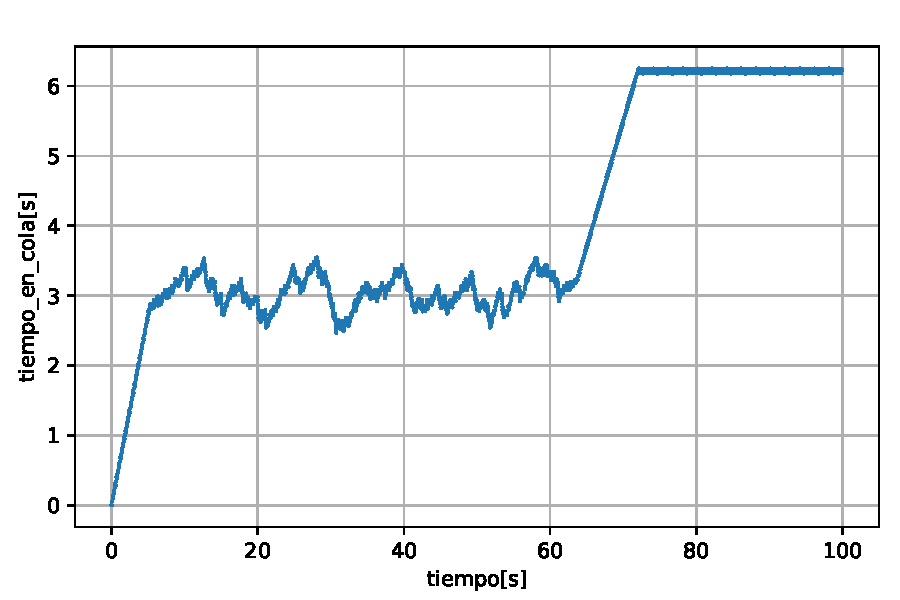
\includegraphics{graficas/sinQoS/tiempo_en_cola_sinQoS.pdf}
        \caption{Tiempo paquetes en cola del router sin QoS}
        \label{fig:sinqos_time}
    \end{figure}

    Como se puede ver en la gráfica \ref{fig:sinqos_time}, hay una oscilación hasta los 60 segundos ya que es cuando se dejan de transmitir los paquetes VoIP. Esa oscilación
    se debe a que los paquetes de voz son mas ligeros que los de UDP, por lo que, hay momentos en que la cola se atasca más ya que a lo
    mejor está liberando los paquetes UDP y otras veces hay una bajada ya que están saliendo los paquetes VoIP
    
    \item ¿Cuál sería la máxima longitud de cola si queremos que el tiempo de encolado de un paquete sea como máximo 1s? \label{item:c}
    
    Para eso vamos a utilizar la ecuación del apartado \ref{item:a}:

    \[
      t_{q} =  \frac{L}{R_{out}} \Rightarrow 1~\mathrm{s} \cdot 34,33~\mathrm{pkts/s} = L \Rightarrow L \approx 35~\mathrm{pkt}
    \]

    Por lo tanto con 35 paquetes como tamaño de la cola, tendremos un encolado de como máximo 1s


\end{enumerate}

\subsection{Para el caso en el que ya solo se están transmitiendo los dos flujos UDP:}
\begin{enumerate}
    
    \item Calcula el tiempo medio en cola de un paquete cuando la cola está llena.
    
    Cuando se deja transmitir VoIP, la tasa de salida de la cola es de:
    \[
      R_{out} = \frac{16000~\text{B/s}}{1000~\text{B/pkts}} = 16~\text{pkts/s}
    \]

    Por lo que el tiempo medio cuando la cola está llena y solo se transmite UDP:
    \[
      t_{q} = \frac{L}{R_{out}} = \frac{100~\mathrm{pkt}}{16~\mathrm{pkts/s}} = 6,25~\mathrm{s}
    \]

    \item ¿Por qué ahora la gráfica no presenta oscilaciones en torno al valor medio?
    
    Como vimos en la gráfica \ref{fig:sinqos_time}, después de 60s (tiempo que solo hay paquetes UDP), no hay ninguna oscilación
    ya que los paquetes son todos de igual tamaño por lo que todos tardan el mismo tiempo en enviarse.
  

\end{enumerate}


\section{Retardo de extremo a extremo}

\subsection{¿Cuál es la relación con la gráfica de tiempo de encolado en el router?}

\begin{figure}[!ht]
    \centering
    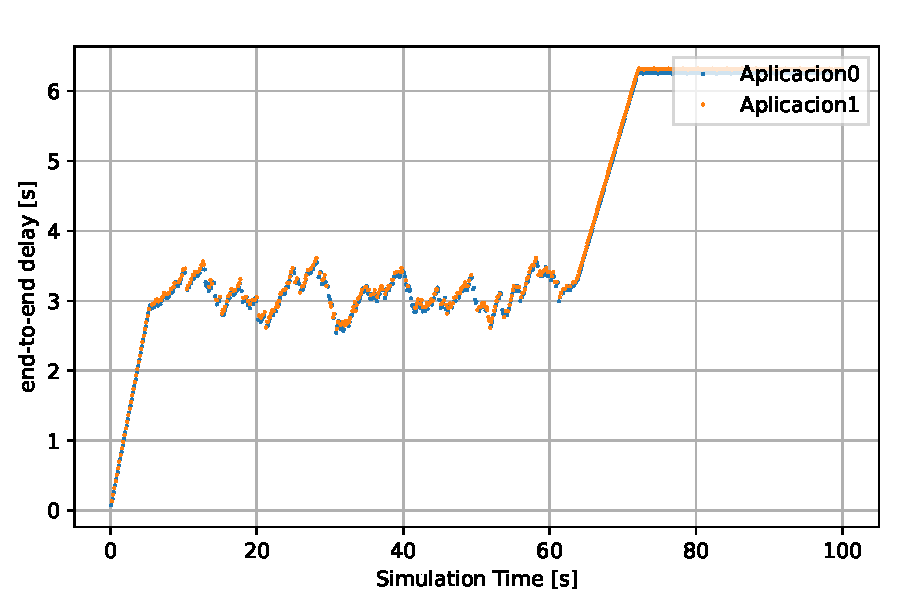
\includegraphics{graficas/sinQoS/ end_to_end__delay_sinQoS.pdf}
    \caption{Retardo extremo a extremos del router sin QoS}
    \label{fig:sinqos_endtoend}
\end{figure}

Hay una relación clara entre el retardo extremo a extremo y el tiempo de encolado de paquetes. Esto se debe a 
que el enlace router-servidor es el único del sistema que sufre problemas de congestión. Por tanto, esto, sumado
a que el sistema es relativamente pequeño (La distancia origen-destino es baja), hace que sea 
evidente pensar que casi todo el retraso de los paquetes proviene del tiempo que pasan dentro 
de esta cola, aumentando el tiempo de llegada de esos paquetes al destino. Por ello, coinciden de 
una forma similar los tiempos de la gráfica \ref{fig:sinqos_time} con respeto a la gráfica \ref{fig:sinqos_endtoend}.


\section{Muestras VoIP y Paquetes VoIP perdidos}

\subsection{¿Por qué se pierde un número constante de muestras al principio? Relaciona con la gráfica de paquetes
perdidos.}

El número constante de muestras que se pierden al principio (ver gráfica \ref{fig:sinqos_lostsamples}) es consecuencia de que la cola se llena muy 
rápidamente al enviar cada 20ms paquetes VoIP, por lo que todos los paquetes que entran se descartan (ver gráfica \ref{fig:sinqos_lostpkts}) y hace que 
las muestras de voz se pierdan de forma uniforme. Una vez que la cola ya está llena, se sigue perdiendo paquetes y con ello muestras, pero deja de ser tan constante ya que se
va procesando poco a poco el tráfico entonces al irse liberando paquetes, hay momentos en los que se pierden más y otros momentos 
en los que se pierden menos.

\begin{figure}[!ht]
  \centering
  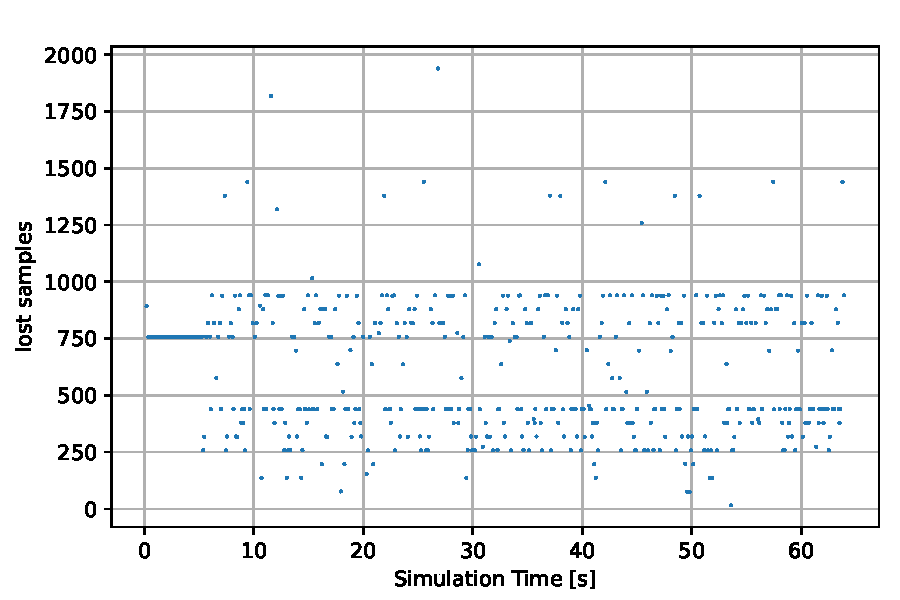
\includegraphics{graficas/sinQoS/ muestras_perdidas_sinQoS.pdf}
  \caption{Muestras perdidas sin QoS}
  \label{fig:sinqos_lostsamples}
\end{figure}

\begin{figure}[!ht]
  \centering
  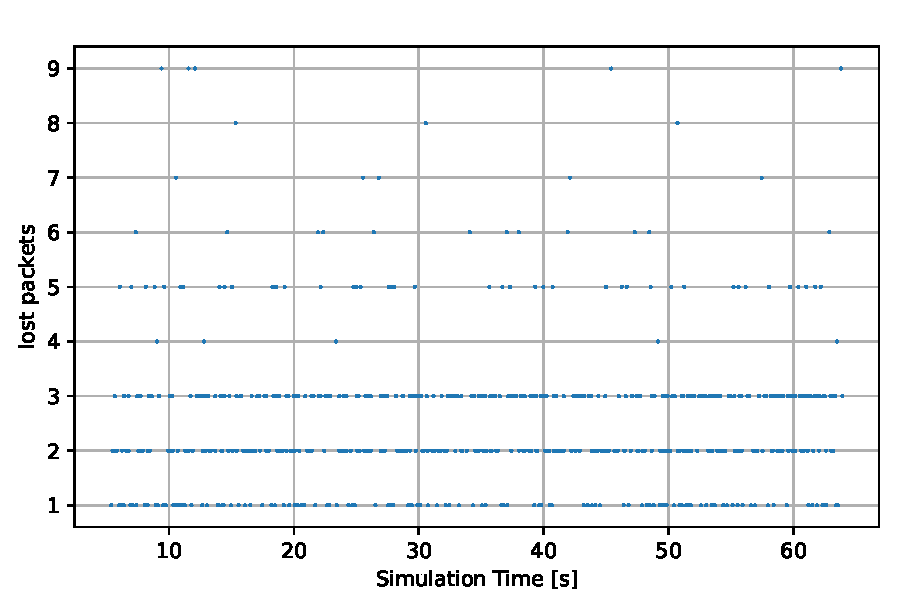
\includegraphics{graficas/sinQoS/paquetes_perdidos_sinQoS.pdf}
  \caption{Retardo extremo a extremos del router sin QoS}
  \label{fig:sinqos_lostpkts}
\end{figure}
 \chapter{Router con QoS - WRR[1,1]}
\label{chap:conqoswrr11}

\tcolorbox[colback=yellow!20, colframe=yellow!50!black, title=Nota]
En este capítulo, como la proporción con WRR[1,1] es igual para ambas colas UDP, en muchos apartados
se da un único resultado para ambas colas, ya que el cálculo y resultado es el mismo para Afx1 que para 
Afx2. Cuando esto ocurre nos referimos a la cola genérica 'Afx'.
\endtcolorbox

\section{Longitud de cola del router}

\subsection{Calcula analíticamente cuántos paquetes habrá como máximo en la cola EF.}

\renewcommand{\theenumi}{\alph{enumi}}

La cola EF, que representa el flujo UDP, es manejada en este caso mediante \textit{Strict Priority Queueing},
por lo que podemos 'ignorar' las colas de paquetes UDP y simplemente calcular la tasa de salida con la
única restricción que supone limitar el tráfico EF a la tasa efectiva resultante de transmitir VoIP que, 
en este caso es de 76,8kbps, como se indica en el enunciado.


\[
R_{InVoIP} = \frac{1~\text{pkt}}{0,02~\text{s}} = 50 ~ \text{pkt/s}
\]

\[
R_{outVoIP} = \frac{76,8~\text{kb/s} \cdot 1000~\text{b/kb} \cdot \frac{1~\text{B}}{8~\text{b}}}{ 192~\text{B/pkt}} = 50~\text{pkt/s}
\]

\[
R_{InVoIP} = R_{outVoIP}
\]

Como la tasa de salida es igual a la de entrada, habrá como mucho un paquete VoIP en
cola en todo momento, ya que cada paquete se transmite al mismo tiempo que llega el siguiente.
Esto puede ratificarse al observar la línea verde, que representa la cola EF, en la figura \ref{fig:wrr11_tam}.

\begin{figure}[!ht]
    \centering
    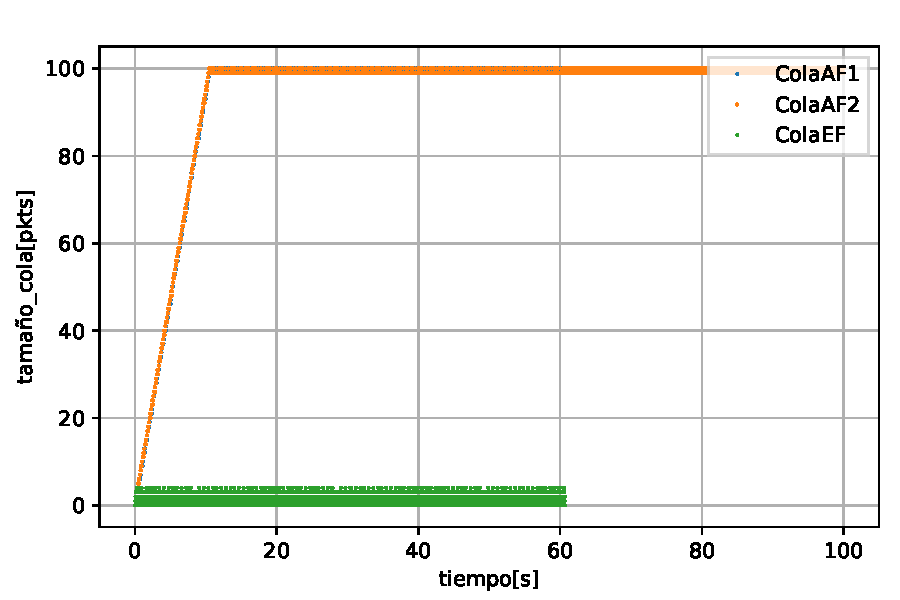
\includegraphics{graficas/DropTail/tamanho_cola_droptail.pdf}
    \caption{Longitud de la cola del router aplicando colas DropTail}
    \label{fig:wrr11_tam}
\end{figure}

\subsection{Mientras dura la transmisión del flujo VoIP:}
\begin{enumerate}
    \item Tasa de salida (en pkt/s y b/s) de cada cola AF1x y AF2x: \\
    \[
        \begin{aligned}
            R_{\text{OutUDP}}[b/s] &= R_{\text{Out}} - R_{\text{OutVoIP}} = 128~\text{kb/s} \cdot 1000~\text{b/kb} - 50~\text{pkt/s} \cdot 199~\text{B/pkt} \cdot 8~\text{b/B} \\
                              &= 48400~\text{b/s} \\
            R_{\text{OutUDP}}[pkt/s] &= 48400~\text{b/s} \cdot \frac{1~\text{B}}{8~\text{b}} \cdot \frac{1~\text{pkt}}{1000~\text{B}} = 6,05~\text{pkt/s} \\ \\
            R_{\text{OutAf1}}[b/s] &= p_{\text{Af1}} \cdot R_{\text{OutUDP}} = \frac{1}{2} \cdot 48400~\text{b/s} = 24200~\text{b/s} \\
            R_{\text{OutAf1}}[pkt/s] &= p_{\text{Af1}} \cdot R_{\text{OutUDP}} = \frac{1}{2} \cdot 6,05~\text{pkt/s} = 3,025~\text{pkt/s} \\ \\
        \end{aligned}
    \]
    \item Paquetes por segundo descartados a la entrada de cada cola:
    \[
        \label{eq:udp_paquetes_descartados_con_VoIP}
        \begin{aligned}
            R_{\text{InAfx}} &= \frac{1~\text{pkt}}{0,08~\text{s}} = 12,5~\text{pkt/s} \\ \\
            Pkt_{\text{DescAfx}} &= R_{\text{InAfx}} - R_{\text{OutAfx}} = 12,5~\text{pkt/s} - 3,025~\text{pkt/s} = 11,636~\text{pkt/s} \\
        \end{aligned}
    \]
    \item Tiempo de llenado de las colas AF1x y AF2x:
    \[
        \begin{aligned}
            t_{\text{FillAfx}} &= \frac{L}{R_{\text{InAfx}} - R_{\text{OutAfx}}} = \frac{100~\text{pkt}}{12,5~\text{pkt/s} - 3,025~\text{pkt/s}} = 9,475~\text{s} \\
        \end{aligned}
    \]
    El resultado de este apartado se puede que es correcto al contrastarlo con la figura \ref{fig:wrr11_tam}.

\end{enumerate}

\vspace{0,3cm}

\subsection{Para el caso en el que ya solo se están transmitiendo los dos flujos UDP, calcula la tasa de entrada [pkt/s] y
tasa de salida [pkt/s].}
La tasa de entrada no cambia. Como se indica en el enunciado, cada cola UDP recibe un paquete cada 80ms. \\
\[
    \begin{aligned}
        R_{\text{InAfx}} &= \frac{1~\text{pkt}}{0,08~\text{s}} = 12,5~\text{pkt/s} \\ \\
    \end{aligned}
\]
Por otra parte, ahora que no hay flujo VoIP (Y suponiendo cola EF vacía), las colas UDP pueden usar todo
el espacio del enlace router-servidor.
\[
    \begin{aligned}
        R_{\text{OutUDP}}[pkt/s] &= 128~\text{kb/s} \cdot 1000~\text{b/kb} \cdot \frac{1~\text{B}}{8~\text{b}} \cdot \frac{1~\text{pkt}}{1000~\text{B}} = 16~\text{pkt/s} \\
		R_{\text{OutAfx}}[pkt/s] &= p_{\text{Afx}} \cdot R_{\text{OutUDP}} = \frac{1}{2} \cdot 16~\text{b/s} = 8~\text{pkt/s} \\
    \end{aligned}
\]
Como se comprueba, el enlace sigue siendo insuficiente y las colas no se vaciarán mientras sigan llegando paquetes
ya que: \[R_{InAfx} > R_{outAfx}\].

\vspace{1cm}

\section{Tiempo en cola del router}

\subsection{Mientras dura la transmisión del flujo VoIP, calcula analíticamente el tiempo en cola de un paquete cuando
las colas AF1x y AF2x están llenas.}
\[
    \begin{aligned}
        t_{\text{qAfx}} &= \frac{L}{R_{\text{OutAfx}}} = \frac{100~\text{pkt}}{3,025~\text{pkt/s}}= 33,058~\text{s} \\
    \end{aligned}
\]

\vspace{0,3cm}

\subsection{Para el caso en el que ya solo se están transmitiendo los dos flujos UDP, calcula el tiempo medio en cola de
un paquete.}
\[
    \begin{aligned}
        t_{\text{qAfx}} &= \frac{L}{R_{\text{OutAfx}}} = \frac{100~\text{pkt}}{8~\text{pkt/s}}= 12,5~\text{s} \\
    \end{aligned}
\]

\vspace{1cm}

\section{Retardo extremo a extremo}

\subsection{Ejercicio 2.3.1}
La explicación es la misma que para el caso del router sin QoS aplicada. Las gráficas de \textit{end-to-end delay}
y tiempo de encolado son prácticamente idénticas debido a que, en el caso de esta práctica, el único segmento del 
sistema donde hay congestión y del que surjen todos los problemas es la conexión router-servidor. Además, el sistema
con el que se trabaja es bastante pequeño, haciendo que apenas se note el tiempo de viaje de los paquetes del origen 
a destino. Por tanto, es evidente ver que la práctica totalidad del retraso de los paquetes proeda del tiempo de 
espera en la cola con la que tratamos en estos ejercicios.

\vspace{1cm}

\section{Muestras VoIP perdidas y Paquetes VoIP perdidos}

\subsection{Ejercicio 2.4.1}

En este caso, las muestras perdidas son muy pocas gracias a aplicar técnicas de QoS. Las pocas muestras
que se pierden pueden ser debidas a ráfagas ocasionales de tráfico u otras situaciones inherentes a la naturaleza de la red.
De hecho, en este caso ya no se pierde ningún paquete en la transmisión.

\begin{figure}[!ht]
    \centering
    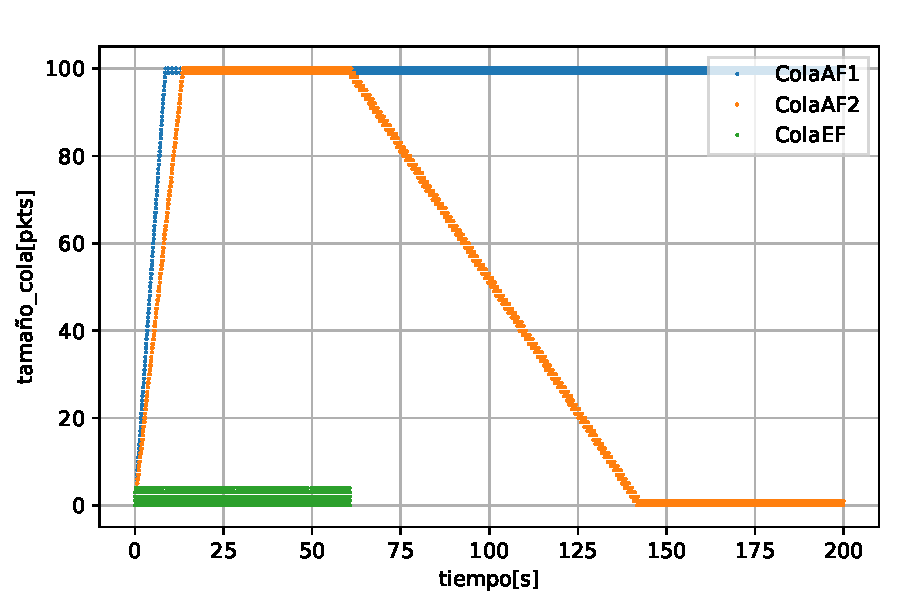
\includegraphics{graficas/WRR/tamao_cola_wrr.pdf}
    \caption{Muestras perdidas en router con WRR[1,1]}
    \label{fig:wrr16_lostsamples}
\end{figure}
 \chapter{Router con QoS - WRR[1,6]}
\label{chap:conqoswrr16}
\renewcommand{\theenumi}{\alph{enumi}}

\tcolorbox[colback=yellow!20, colframe=yellow!50!black, title=Nota]
En este capítulo, aunque la proporción ya no es la misma como en el caso del WRR[1,1], algunos 
cálculos, como la tasa de entrada en cada cola, es equivalente para ambas, por los que nos 
referimos a una única cola genérica 'Afx', que representa ambas colas de tráfico UDP.
\endtcolorbox

\section{Longitud de cola del router}

\subsection{Mientras dura la transmisión del flujo VoIP}
\begin{enumerate}
    \item Tasa de salida (en pkt/s y b/s) de cada cola AF1x y AF2x:
    \[
        \begin{aligned}
            R_{\text{OutUDP}}[b/s] &= R_{\text{Out}} - R_{\text{OutVoIP}} = 128~\text{kb/s} \cdot 1000~\text{b/kb} - 50~\text{pkt/s} \cdot 199~\text{B/pkt} \cdot 8~\text{b/B} \\
                              &= 48400~\text{b/s} \\
            R_{\text{OutUDP}}[pkt/s] &= 48400~\text{b/s} \cdot \frac{1~\text{B}}{8~\text{b}} \cdot \frac{1~\text{pkt}}{1000~\text{B}} = 6,05~\text{pkt/s} \\ \\
            R_{\text{OutAf1}}[b/s] &= p_{\text{Af1}} \cdot R_{\text{OutUDP}} = \frac{1}{7} \cdot 48400~\text{b/s} = 6914~\text{b/s} \\
            R_{\text{OutAf1}}[pkt/s] &= p_{\text{Af1}} \cdot R_{\text{OutUDP}} = \frac{1}{7} \cdot 6,05~\text{pkt/s} = 0,864~\text{pkt/s} \\ \\
            R_{\text{OutAf2}}[b/s] &= p_{\text{Af2}} \cdot R_{\text{OutUDP}} = \frac{6}{7} \cdot 48400~\text{b/s} = 41486~\text{b/s} \\
            R_{\text{OutAf2}}[pkt/s] &= p_{\text{Af2}} \cdot R_{\text{OutUDP}} = \frac{6}{7} \cdot 6,05~\text{pkt/s} = 5,186~\text{pkt/s} \\
        \end{aligned}
    \]
    En este caso, a diferencia del capítulo anterior (WRR[1,1]), al tener pesos distintos para cada cola,
    la tasa de salida de la cola es mucho mayor en Afx2 que en Afx1.
    \item Paquetes por segundo descartados a la entrada de cada cola:
    \[
        \begin{aligned}
            R_{\text{InAfX}} &= \frac{1~\text{pkt}}{0,08~\text{s}} = 12,5~\text{pkt/s} \\ \\
            Pkt_{\text{DescAf1}} &= R_{\text{InAf1}} - R_{\text{OutAf1}} = 12,5~\text{pkt/s} - 0,864~\text{pkt/s} = 11,636~\text{pkt/s} \\
            Pkt_{\text{DescAf2}} &= R_{\text{InAf2}} - R_{\text{OutAf2}} = 12,5~\text{pkt/s} - 5,186~\text{pkt/s} = 7,314~\text{pkt/s} \\
        \end{aligned}
    \]
    \item Tiempo de llenado de las colas AF1x y AF2x:
    \[
        \begin{aligned}
            t_{\text{FillAf1}} &= \frac{L}{R_{\text{InAf1}} - R_{\text{OutAf1}}} = \frac{100~\text{pkt}}{12,5~\text{pkt/s} - 0,864~\text{pkt/s}} = 8,594~\text{s} \\
            t_{\text{FillAf2}} &= \frac{L}{R_{\text{InAf2}} - R_{\text{OutAf2}}} = \frac{100~\text{pkt}}{12,5~\text{pkt/s} - 5,186~\text{pkt/s}} = 13,672~\text{s} \\
        \end{aligned}
    \]
    Como se observa en la figura \ref{fig:wrr16_tam}, el tiempo de llenado paras las colas UDP es muy 
    bajo, coincidiendo con lo calculado en este apartado.
\end{enumerate}
\begin{figure}[!ht]
    \centering
    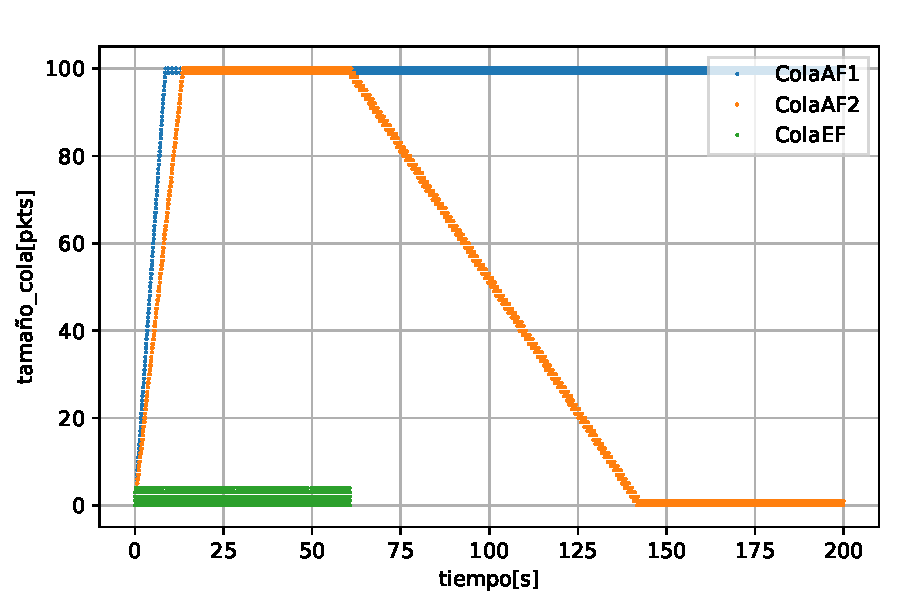
\includegraphics{graficas/WRR/tamao_cola_wrr.pdf}
    \caption{Tamaño de la cola en router con WRR[1,6]}
    \label{fig:wrr16_tam}
\end{figure}

\vspace{0,3cm}

\subsection{Para el caso en el que ya solo se están transmitiendo los dos flujos UDP, calcula la tasa de entrada [pkt/s] y
tasa de salida [pkt/s].}
\[
    \begin{aligned}
        R_{\text{InAfX}} &= \frac{1~\text{pkt}}{0,08~\text{s}} = 12,5~\text{pkt/s} \\ \\
        R_{\text{OutUDP}}[pkt/s] &= 128~\text{kb/s} \cdot 1000~\text{b/kb} \cdot \frac{1~\text{B}}{8~\text{b}} \cdot \frac{1~\text{pkt}}{1000~\text{B}} = 16~\text{pkt/s} \\ \\
        R_{\text{OutAf1}}[pkt/s] &= p_{\text{Af1}} \cdot R_{\text{OutUDP}} = \frac{1}{7} \cdot 16~\text{pkt/s} = 2,286~\text{pkt/s} \\
        R_{\text{OutAf2}}[pkt/s] &= p_{\text{Af2}} \cdot R_{\text{OutUDP}} = \frac{6}{7} \cdot 16~\text{pkt/s} = 13,714~\text{pkt/s} \\
    \end{aligned}
\]
Es interesante fijarse que, para este contexto, al tener un peso de 6, la cola Afx2 se comienza a vaciar 
cuando cesa el flujo VoIP como puede verse con lo que se acaba de calcular (La tasa de salida de Afx2 es mayor 
que la tasa de entrada en la misma). También se refleja en la figura \ref{fig:wrr16_tam}.

\vspace{1cm}

\section{Tiempo en cola del router}
\subsection{Mientras dura la transmisión del flujo VoIP, calcula analíticamente el tiempo en cola de un paquete cuando
la cola AF2x está llena.}
\[
    \begin{aligned}
        t_{\text{qAf2}} &= \frac{L}{R_{\text{OutAf2}}} = \frac{100~\text{pkt}}{5,186~\text{pkt/s}}= 19,283~\text{s} \\
    \end{aligned}
\]
Para comprobar este resultado podemos acudir a la figura \ref{fig:wrr16_time} para ver como el tiempo 
en cola de los paquetes de Afx2 efectivamente se estanca justo antes de los 20s.

\vspace{0,3cm}

\subsection{¿En qué instante entró en la cola AF1x el paquete que salió en t = 60s? ¿Estaba la cola AF1x llena cuando
entró?}
Para realizar este ejercicio nos ayudaremos de la gráfica correspondiente, ya que no es posible 
realizarlo analíticamente, al menos con los conocimientos que tenemos actualmente. Observando 
la figura \ref{fig:wrr16_time} desde Omnet, podemos ver que el paquete saliente de la cola Af1x en el segundo 60, lleva 
en cola un tiempo aproximado de 55,1s.
\[
    \begin{aligned}
        t_{\text{in}} &= t_{\text{out}} - t_{\text{qAf1}} = 60~\text{s} - 55,1~\text{s}= 4,9~\text{s} \\
    \end{aligned}
\]
Por tanto, el momento en el que entró, fue el segundo 4,9. Si nos fijamos en la figura \ref{fig:wrr16_tam}, la cola aún no estaba llena.

\vspace{0,3cm}

\subsection{¿En qué instante salió el primer paquete que se encontró la cola AF1x llena?}
Aunque podría haber forma de obtener un resultado aproximado calculándolo analíticamente, la forma
que se usará para resolver este ejercicio es, igual que en el anterior, la comparación con las gráficas en Omnet.
Primero, acudiremos a la figura \ref{fig:wrr16_tam}. En ella, vemos que el primer paquete que encontró la cola llena
lo hizo en el instante t=8,6s. 
A continuación, debemos buscar el punto en la cola Afx1 de la figura \ref{fig:wrr16_time} en el que,
si  restamos la componente X a la Y, resulte 8,6. Este punto coincidiría con el instante t=84s, momento
en el que salió el primer paquete que encontró la cola llena.

\begin{figure}[!ht]
    \centering
    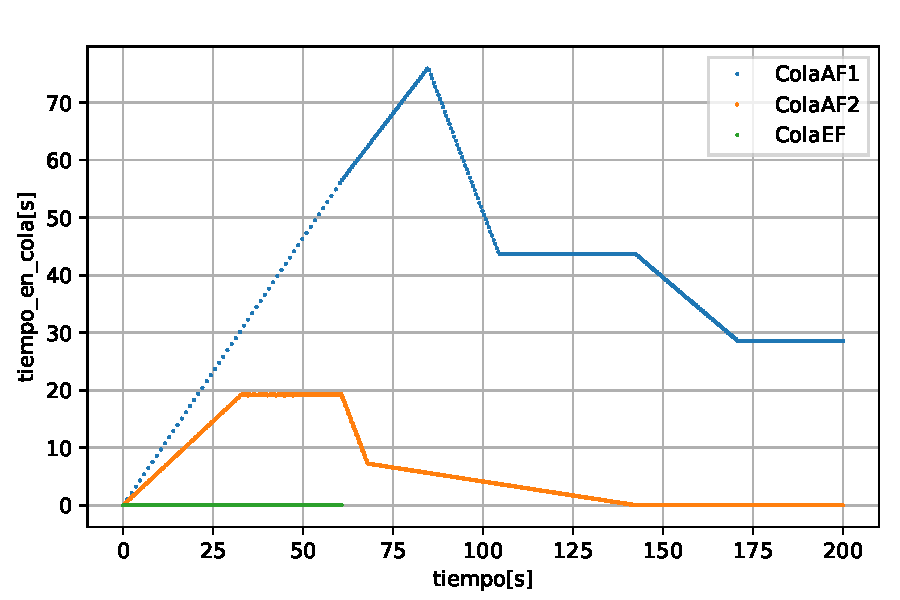
\includegraphics{graficas/WRR/tiempo_en_cola_wrr.pdf}
    \caption{Tiempo en cola de paquetes en router con WRR[1,6]}
    \label{fig:wrr16_time}
\end{figure}


 \chapter{Router con QoS - Colas RED}
\label{chap:colasRED}

\section{Longitud de cola del router}

\subsection{Explica por qué se llenan tanto la cola AF1x como la AF2x pese a usar el algoritmo RED.} \label{chap:ejercicio411}
Como se puede ver en la gráfica \ref{fig:colasRED_tam} y en el archivo .ini de la práctica, la cola \textbf{AFX1} tiene un umbral máximo de 100 paquetes y la cola
\textbf{AFX2} tiene un umbral máximo de 50 paquetes. Además la probabilidad de descarte de paquetes es de 0,5 y 1 respectivamente en cada una.

Ambas colas tienen también un factor de suavizado que se usa para calcular el promedio de la longitud de la cola y ajustar dinámicamente la probabilidad
de descarte de paquetes. Cuanto menor sea este factor, el cálculo de la longitud promedio de la cola se hará de forma mas lenta. 
Ese factor es de 0,03 en la cola \textbf{AFX1} y de 0,01 en la cola \textbf{AFX2}.

Como en este escenario hay una alta cantidad de paquetes entrantes, este factor de suavizado es muy bajo para este tráfico por lo que las colas tardan en detectar
la congestión y se llenan. Además en la cola \textbf{AFX1}, como la probabilidad de descarte es del 100\%, cuando la cola se llena se ve una
bajada muy grande en el tamaño, ya que en ese momento cualquier paquete que entre se descarta hasta que la cola quede estabilizada. 


\begin{figure}[!ht]
    \centering
    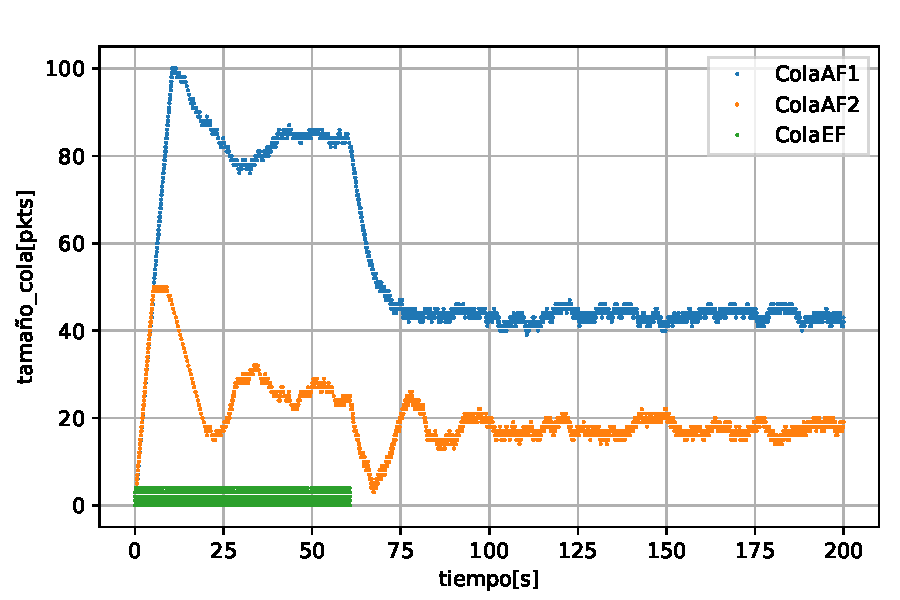
\includegraphics{graficas/RED/tamao_cola_red.pdf}
    \caption{Longitud cola del router con QoS usando colas RED}
    \label{fig:colasRED_tam}
\end{figure}


\subsection{Explica a qué es debida la bajada del tamaño de la cola AF2x:}
\begin{enumerate}
    \item Mientras dura la transmisión VoIP.
    
    Como se explicó en el apartado \ref{chap:ejercicio411}, al llenarse la cola la probabilidad de descarte es la máxima, por lo que se descartan
    todos los paquetes que llegan a la cola, bajando así la congestión del tráfico.      

    \item Cuando ya no hay transmisión VoIP.
    
    A partir de los 60s se deja de transmitir paquetes VoIP entonces queda libre todo el ancho de banda para los paquetes UDP, 
    lo que hace que las colas estén ya menos congestionadas. Aún así, se ven subidas y bajadas en el tamaño de la cola (gráfica \ref{fig:colasRED_tam}) 
    ya que RED sigue descartando paquetes según el factor de suavizado, por lo que se aplica el límite según la longitud promedia de la cola (calculado en 
    el apartado \ref{text:calculos}).
    


\end{enumerate}

\subsection{¿Cuál es la tasa de entrada efectiva que fija el algoritmo RED en cada cola?} \label{text:calculos}

Para calcular la tasa de entrada efectiva, vamos a calcular el longitud promedia de la cola y a partir de ella, la tasa efectiva:

Longitud promedia, según la documentación de inet:

\[
\text{avg} = (1 - w_q) \cdot \left(\frac{\text{maxth} - \text{minth}}{2}\right) + w_q \cdot \text{qlen}
\]

Cola (\textbf{AFX1}):
\[
 avg_{afx1} = (1-0,03) \cdot \left((100-10)/2\right) + 0.03 \cdot 100 = 43,65 + 3 = 46,65 [pkts]
\]

Cola (\textbf{AFX2}):
\[
 avg_{afx2} = (1-0,01) \cdot \left((50-10)/2\right) + 0.01 \cdot 50 = 19,8 + 0,5 = 20,3 [pkts]
\]

Una vez tenemos la longitud promedia, vamos a calcular la probabilidad de descarte de un paquete:

\[
P(descarte) = \text{maxP} \cdot \left(\frac{\text{avg} - \text{minth}}{\text{maxth} - \text{minth}}\right)
\]

Cola (\textbf{AFX1}):

\[
P(descarte)_{afx1} = 0,5 \cdot \left(\frac{46,65 - 10}{100 - 10}\right) = 0,2\%
\]

Cola (\textbf{AFX2}):

\[
P(descarte)_{afx2} = 1 \cdot \left(\frac{20,3 - 10}{50 - 10}\right) = 0,2575\%
\]

Una vez tenemos la probabilidad de que un paquete se descarte, podemos calcular la tasa efectiva:

\[
Tasa(efectiva) = \text{maxth} \cdot (1 - P(descarte))
\]

Cola (\textbf{AFX1}): 

\[
Tasa(efectiva)_{afx1} = 100 \cdot (1 - 0,2) = 80 [pkts/s]
\]

Cola (\textbf{AFX2}):

\[
Tasa(efectiva)_{afx2} = 100 \cdot (1 - 0,2575) = 74,25 [pkts/s]
\]


\section{Tiempo en cola del router}
\subsection{Explica a qué es debido el salto en el tiempo de encolado de la cola AF2x.}

El salto se debe a los paquetes que se descartan en ese momento en la cola (ver gráfica \ref{fig:colasRED_time} ). Como la probabilidad de descarte de \textbf{AFX2} 
es del 100\%, todos los paquetes que entran se descartan por lo que al no entrar ningún paquete, los paquetes que están en la cola se liberan 
con más rapidez hasta que la cola se vuelva a llenar.

\begin{figure}[!ht]
    \centering
    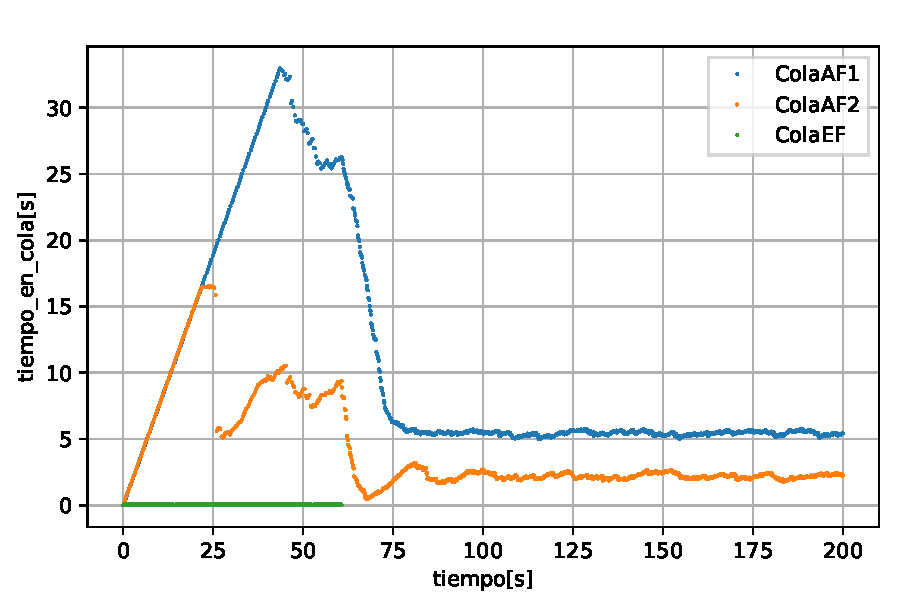
\includegraphics{graficas/RED/tiempo_en_cola_red.pdf}
    \caption{Tiempo encolado cola del router con QoS usando colas RED}
    \label{fig:colasRED_time}
\end{figure}

\subsection{Explica las ventajas e inconvenientes del comportamiento de cada cola AF1x y AF2x. }

En la cola \textbf{AFX1}, la ventaja es que al tener el umbral máximo alto, el número de paquetes que se pierden es bajo y además tiene una probabilidad
de descarte flexible. Como inconveniente, el tiempo de encolado de paquetes es mayor que \textbf{AFX2}, por lo se tardan más en transmitir.

Con respeto a la cola \textbf{AFX2}, la principal ventaja es el tiempo de encolado, ya que es bajo. 
Los inconvenientes son que, al principio, el número de paquetes decartados son muy seguidos ya que tiene una alta probabilidad de descarte y además el
umbral máximo está por debajo del tamaño de la cola por lo que se están desperdiciando recursos y, como conseuencia, la cola se llena más rápido.
 


 \chapter{Otras Gráficas}
\label{chap:sinqos}

\begin{figure}[!ht]
    \centering
    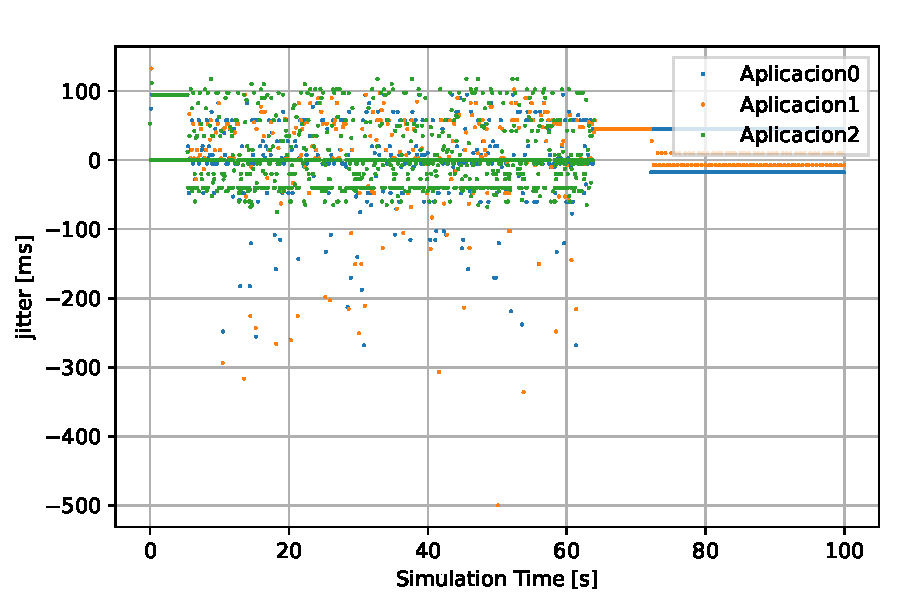
\includegraphics{graficas/sinQoS/jitter_SinQoS.pdf}
    \caption{Jitter a partir retardo extremo a extremo del router sin QoS}
    \label{fig:sinqos_jitter}
\end{figure}

\begin{figure}
    \centering
    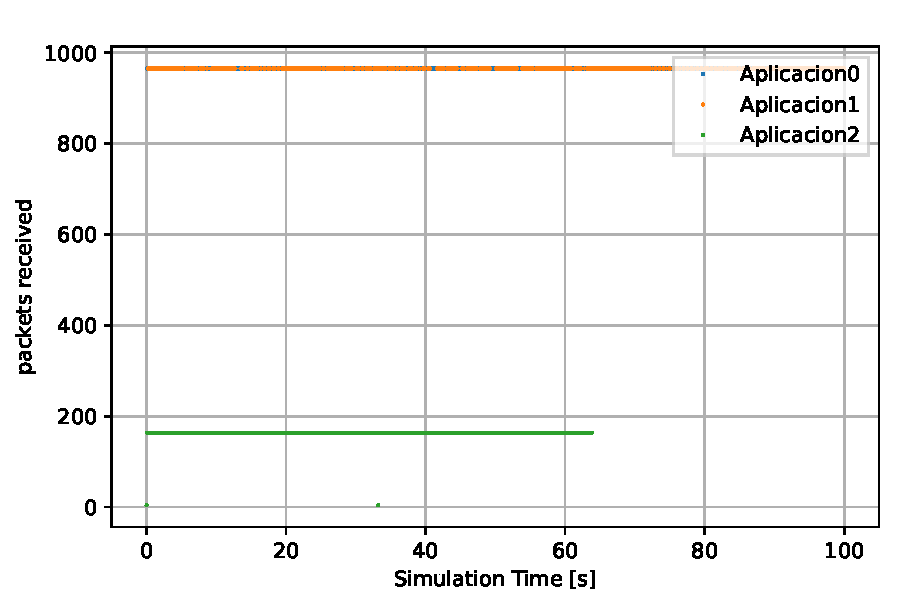
\includegraphics{graficas/sinQoS/packetsReceived_sinQoS.pdf}
    \caption{Paquetes recibidos en el servidor sin QoS}
    \label{fig:sinqos_pktreceived}
\end{figure}

\begin{figure}
    \centering
    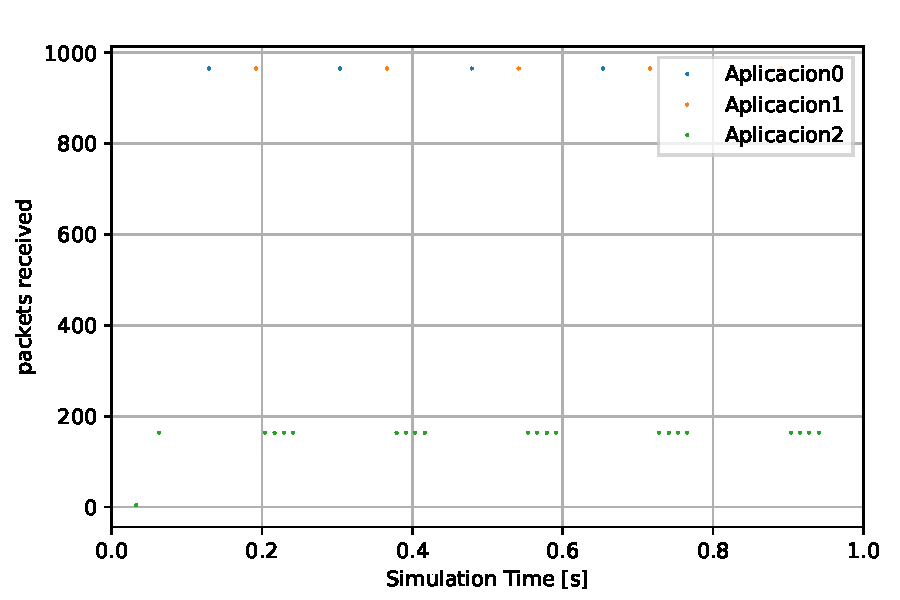
\includegraphics{graficas/sinQoS/packetsReceived_sinQoS_1.pdf}
    \caption{Paquetes recibidos en el servidor sin QoS intervalo 0-1}
    \label{fig:sinqos_pktreceived01}
\end{figure}

\begin{figure}
    \centering
    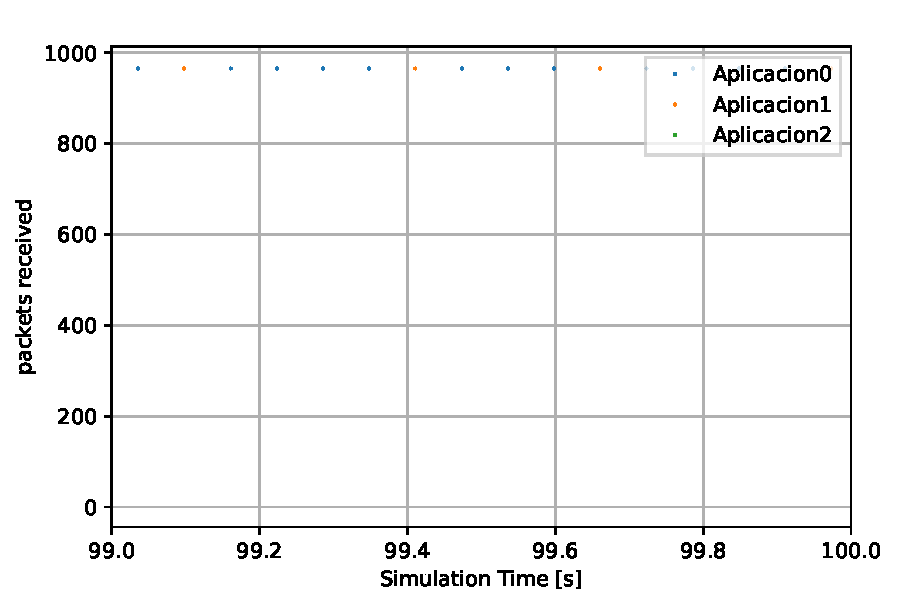
\includegraphics{graficas/sinQoS/packetsReceived_sinQoS_99.pdf}
    \caption{Paquetes recibidos en el servidor sin QoS intervalo 99-100}
    \label{fig:sinqos_pktreceived99100}
\end{figure}


\begin{figure}[!ht]
    \centering
    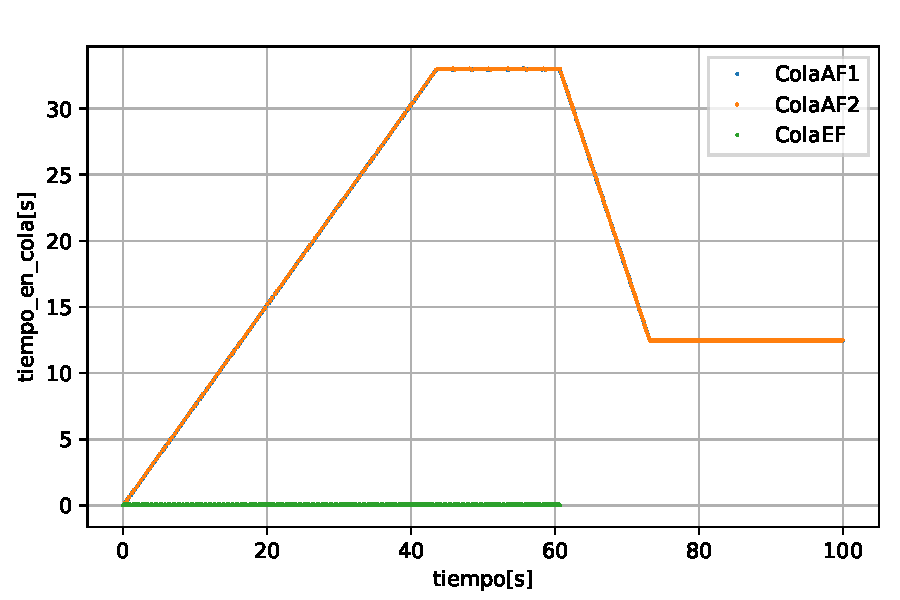
\includegraphics{graficas/DropTail/tiempo_en_cola_droptail.pdf}
    \caption{Tiempo encolado droptail}
    \label{fig:droptail_time}
\end{figure}

\begin{figure}
    \centering
    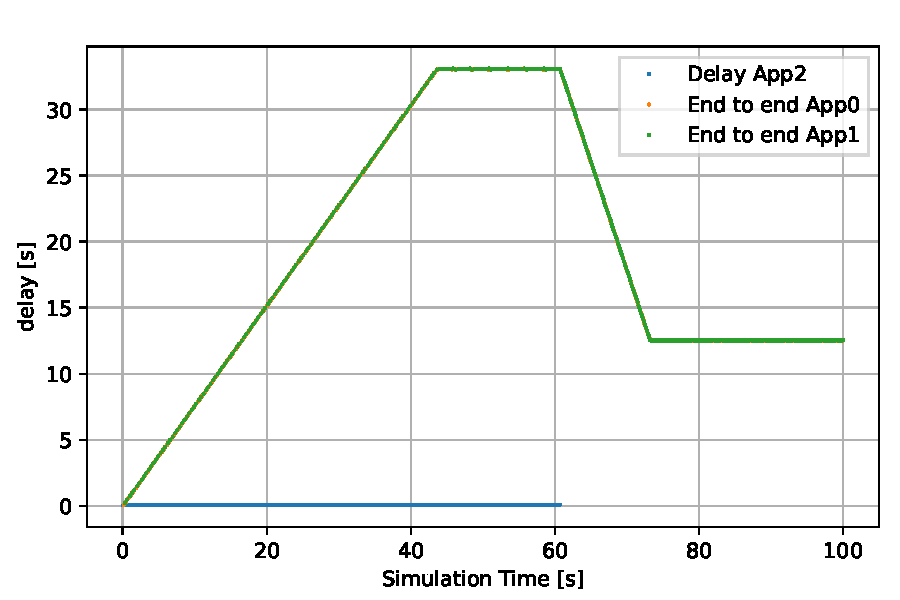
\includegraphics{graficas/DropTail/delay_DT.pdf}
    \caption{Delay extremo a extremo con droptail}
    \label{fig:sinqos_pktreceived99100}
\end{figure}

\begin{figure}
    \centering
    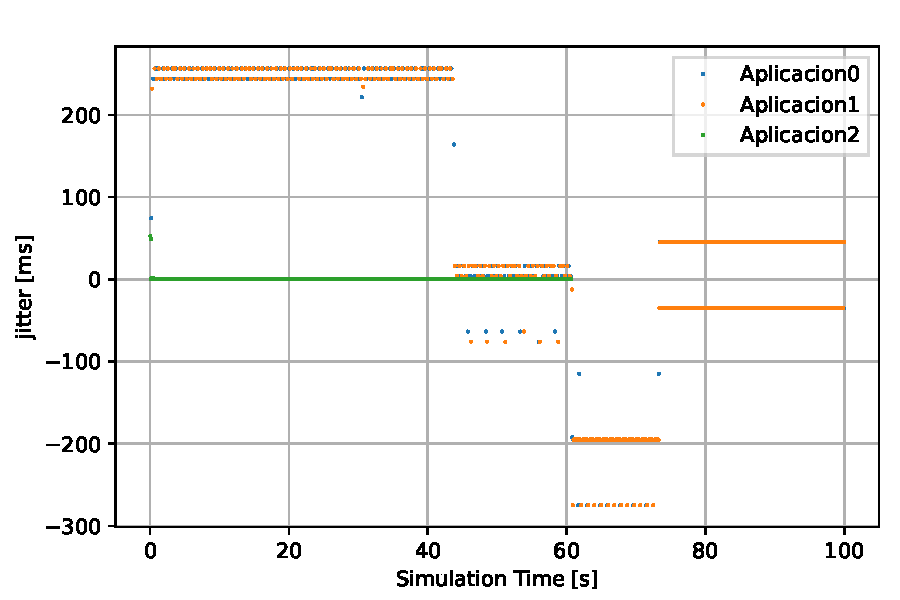
\includegraphics{graficas/DropTail/jitter_DT.pdf}
    \caption{Jitter a partir retardo extremo a extremo droptail}
    \label{fig:sinqos_pktreceived99100}
\end{figure}

\begin{figure}
    \centering
    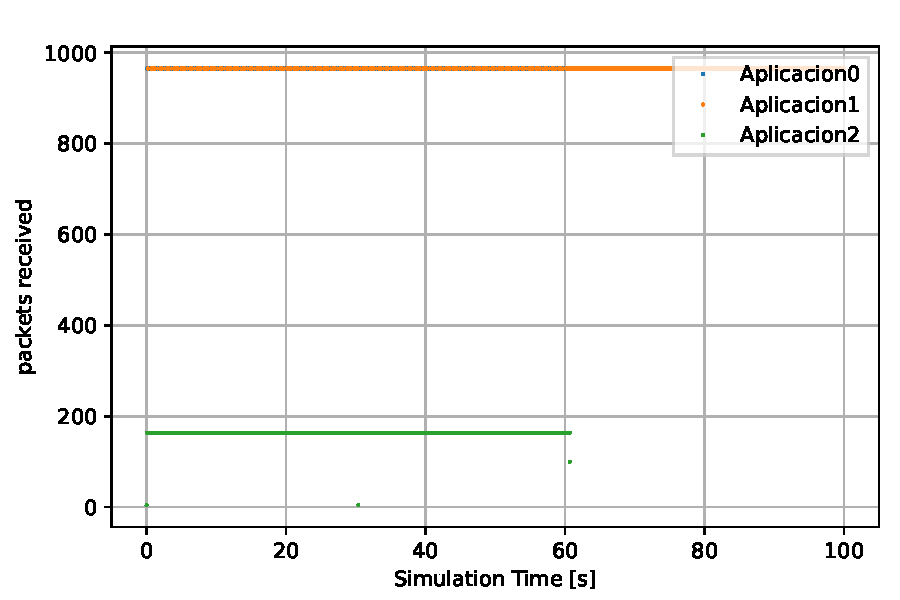
\includegraphics{graficas/DropTail/packetsReceived_DT.pdf}
    \caption{Paquetes recibidos en el servidor droptail}
    \label{fig:sinqos_pktreceived99100}
\end{figure}

\begin{figure}
    \centering
    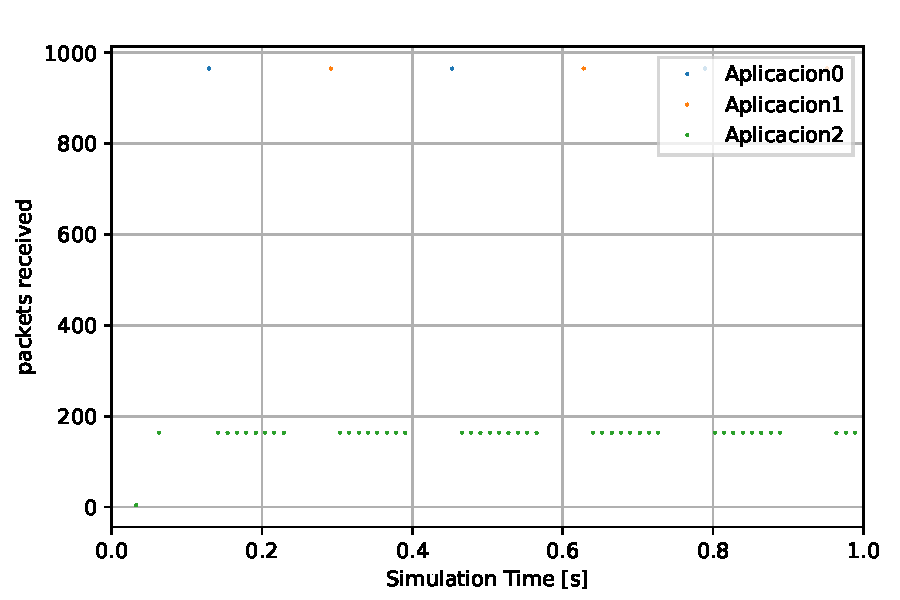
\includegraphics{graficas/DropTail/packetsReceived_DT_1.pdf}
    \caption{Paquetes recibidos en el sevidor droptail intervalo 0-1 }
    \label{fig:sinqos_pktreceived99100}
\end{figure}

\begin{figure}
    \centering
    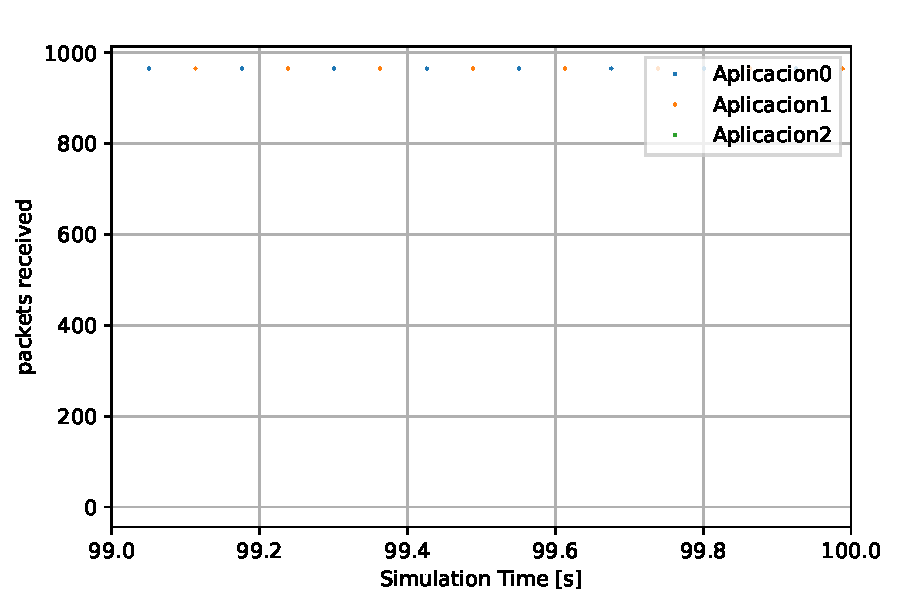
\includegraphics{graficas/DropTail/packetsReceived_DT_99.pdf}
    \caption{Paquetes recibidos en el servidor droptail intervalo 99-100}
    \label{fig:sinqos_pktreceived99100}
\end{figure}


\begin{figure}[!ht]
    \centering
    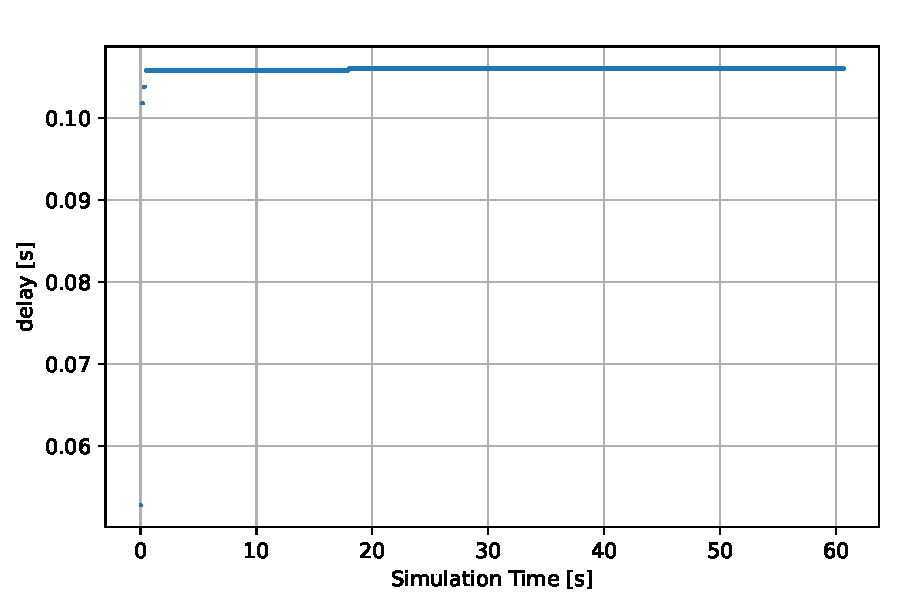
\includegraphics{graficas/WRR/delay_wrr.pdf}
    \caption{Retardo extremo a extremo WRR16}
    \label{fig:sinqos_pktreceived99100}
\end{figure}

\begin{figure}
    \centering
    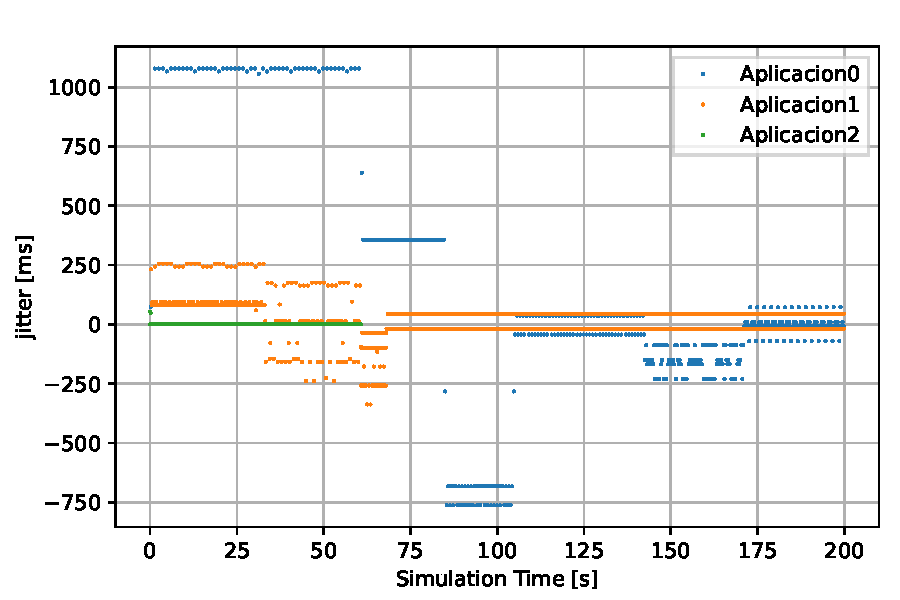
\includegraphics{graficas/WRR/jitter_WRR.pdf}
    \caption{Jitter a partir retardo extremo a extremo WRR16}
    \label{fig:sinqos_pktreceived99100}
\end{figure}

\begin{figure}
    \centering
    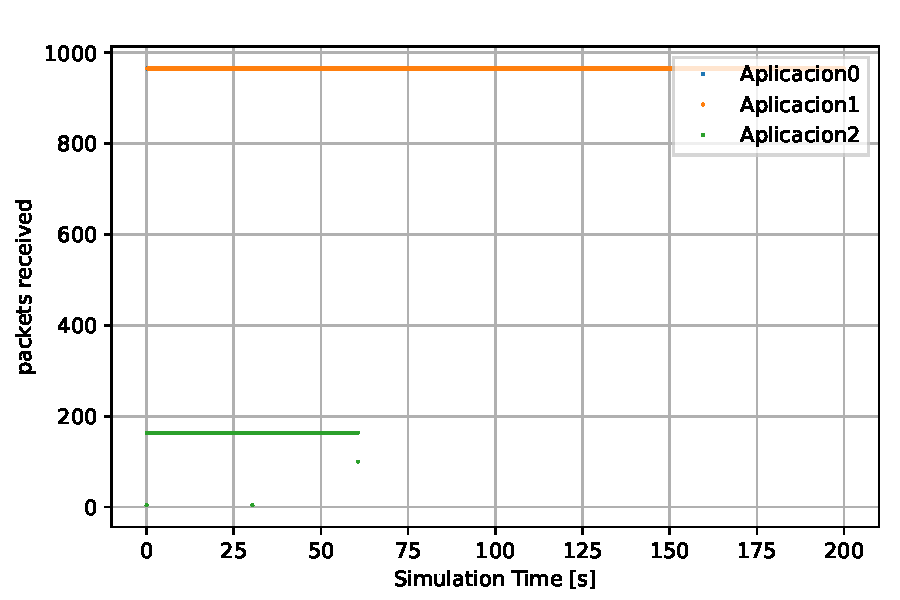
\includegraphics{graficas/WRR/packetsReceived_WRR.pdf}
    \caption{Paquetes recibidos en el servidor con WRR16}
    \label{fig:sinqos_pktreceived99100}
\end{figure}

\begin{figure}
    \centering
    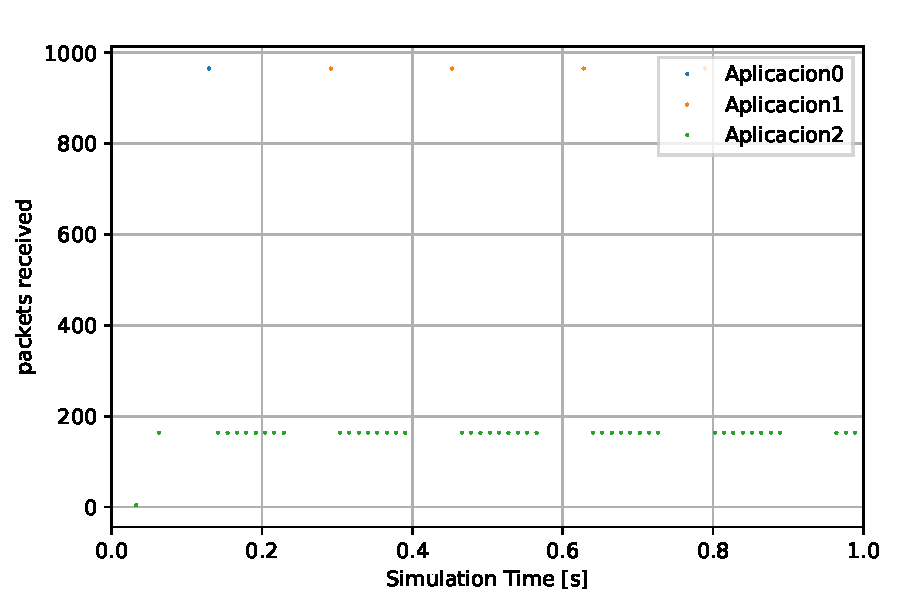
\includegraphics{graficas/WRR/packetsReceived_WRR_1.pdf}
    \caption{Paquetes recibidos en el servidor con WRR16 intervalo 0-1}
    \label{fig:sinqos_pktreceived99100}
\end{figure}

\begin{figure}
    \centering
    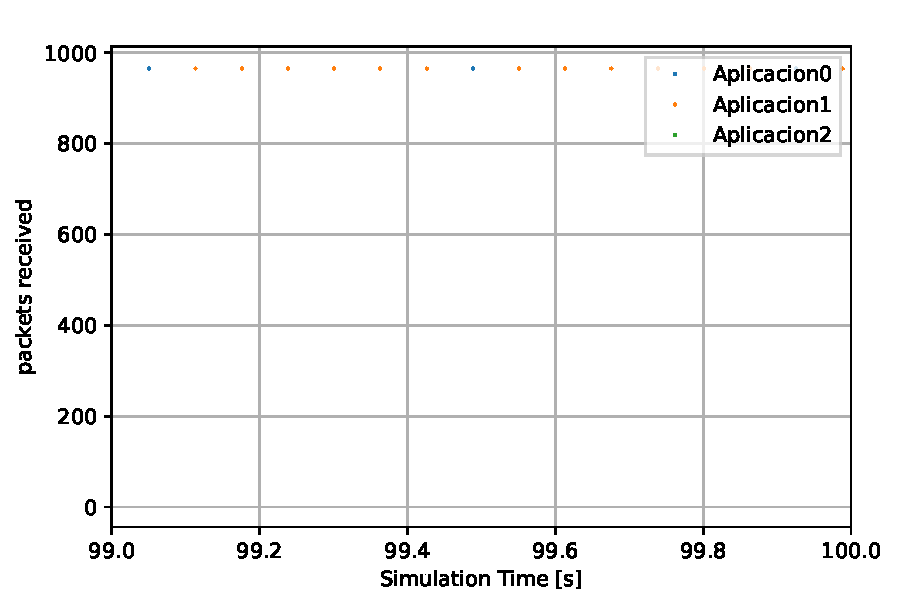
\includegraphics{graficas/WRR/packetsReceived_WRR_99.pdf}
    \caption{Paquetes recibidos en el servidor con WRR16 intervalo 99-100}
    \label{fig:sinqos_pktreceived99100}
\end{figure}

\begin{figure}
    \centering
    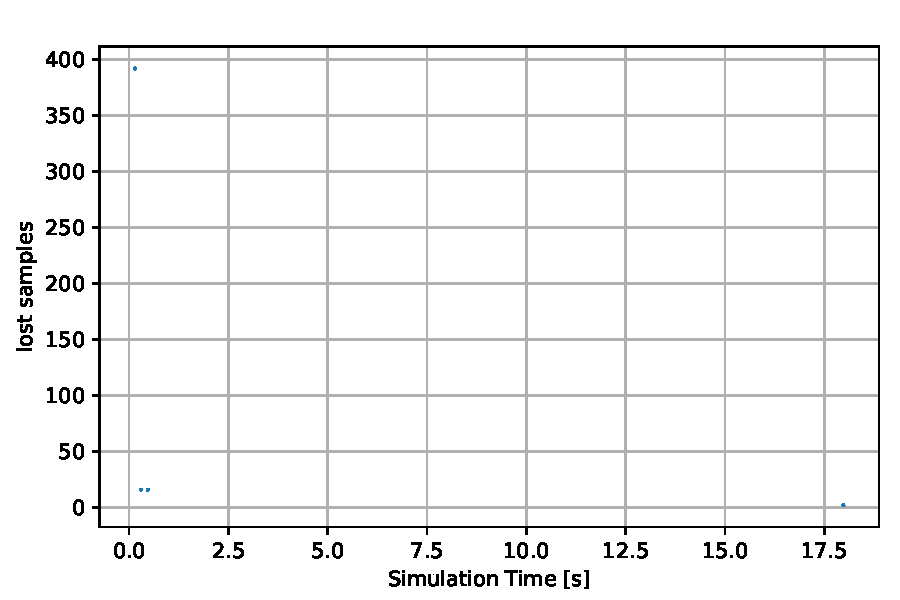
\includegraphics{graficas/WRR/muestras_perdidas_wrr.pdf}
    \caption{Muestras perdidas WRR16}
    \label{fig:sinqos_pktreceived99100}
\end{figure}


\begin{figure}[!ht]
    \centering
    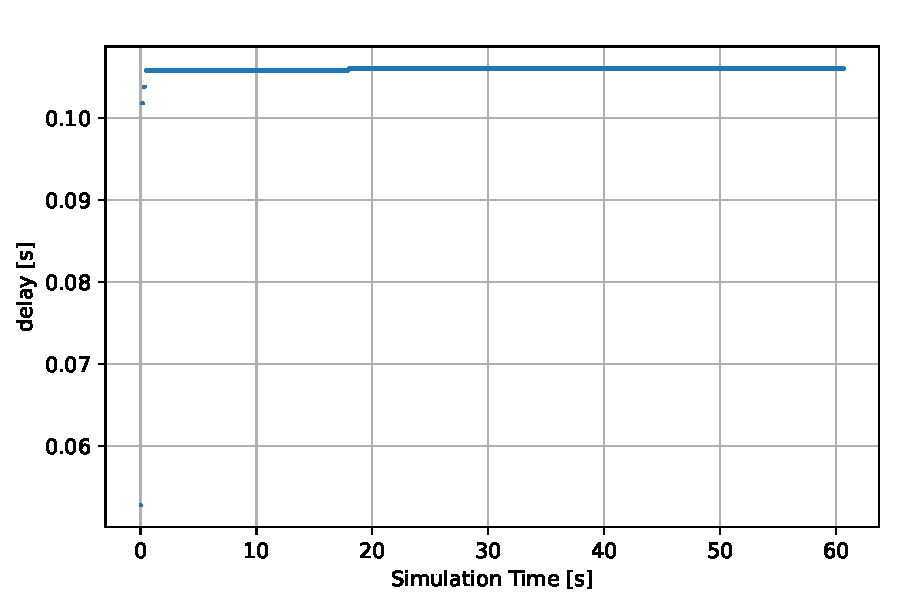
\includegraphics{graficas/RED/delay_red.pdf}
    \caption{Retardo extremo a extremo RED}
    \label{fig:sinqos_pktreceived99100}
\end{figure}

\begin{figure}
    \centering
    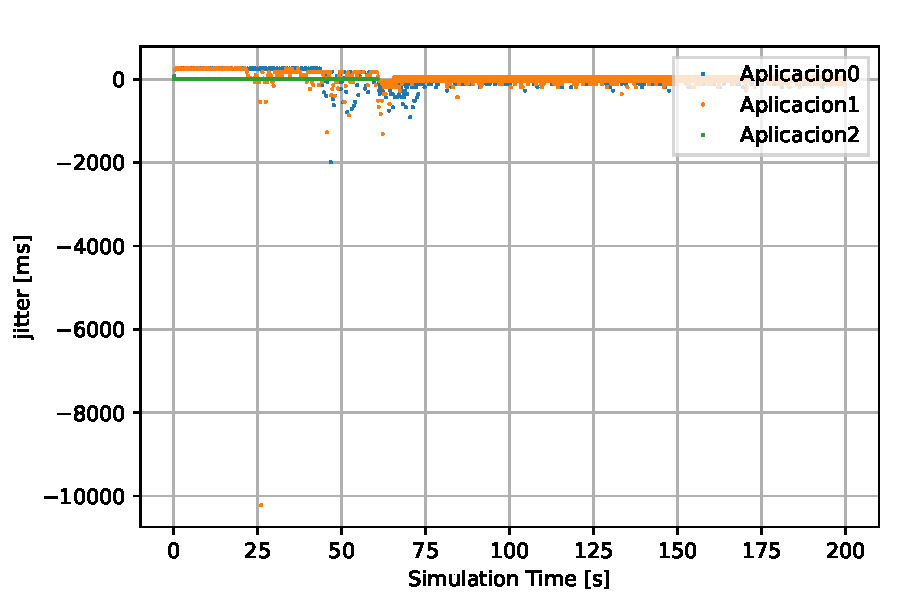
\includegraphics{graficas/RED/jitter_RED.pdf}
    \caption{Jitter a partir retardo extremo a extremo RED}
    \label{fig:sinqos_pktreceived99100}
\end{figure}

\begin{figure}
    \centering
    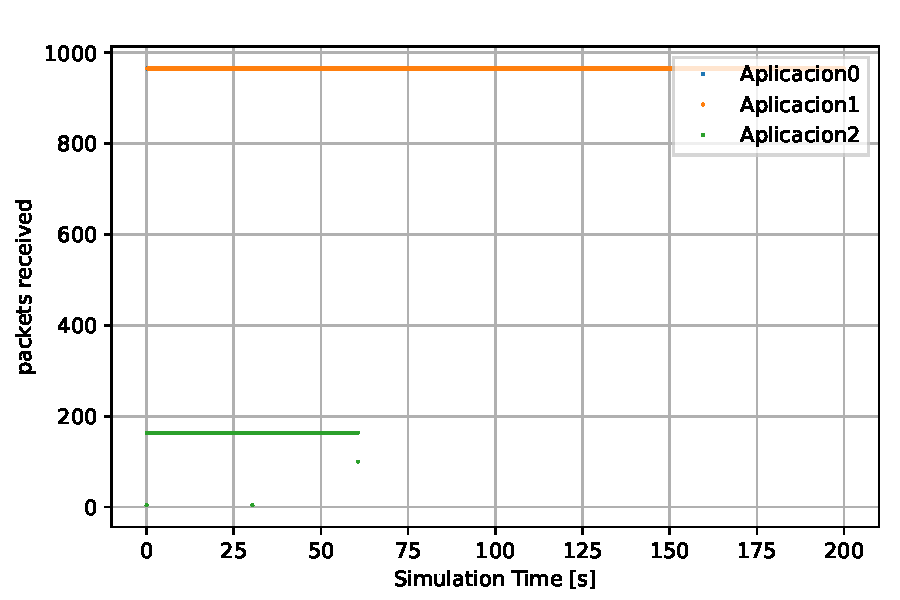
\includegraphics{graficas/RED/packetsReceived_RED.pdf}
    \caption{Paquetes recibidos en el servidor con RED}
    \label{fig:sinqos_pktreceived99100}
\end{figure}

\begin{figure}
    \centering
    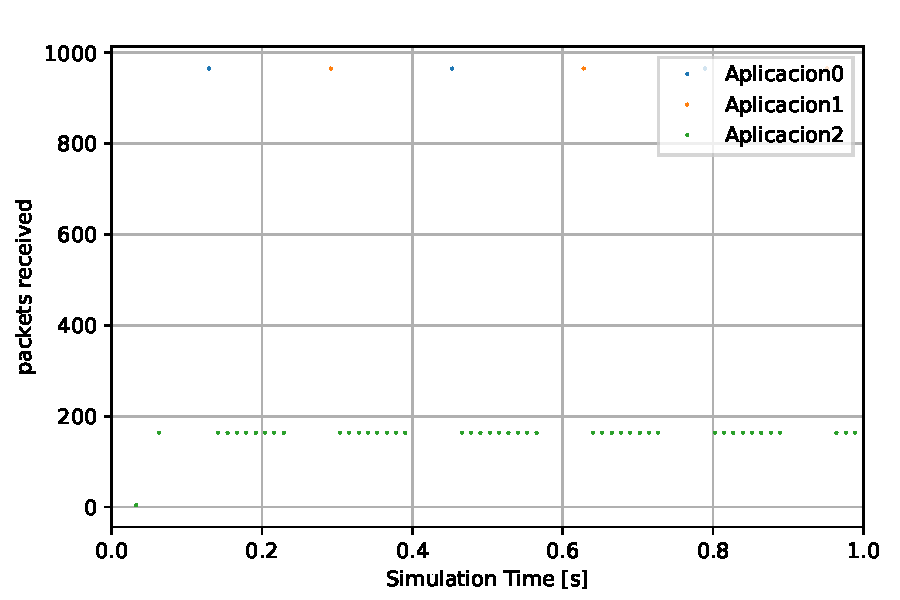
\includegraphics{graficas/RED/packetsReceived_RED_1.pdf}
    \caption{Paquetes recibidos en el servidor con RED intervalo 0-1}
    \label{fig:sinqos_pktreceived99100}
\end{figure}

\begin{figure}
    \centering
    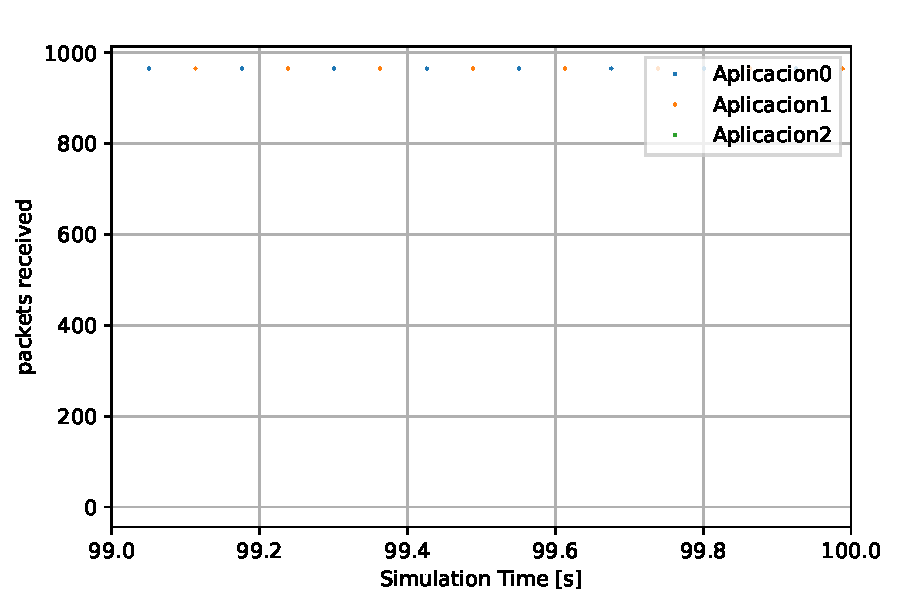
\includegraphics{graficas/RED/packetsReceived_RED_99.pdf}
    \caption{Paquetes recibidos en el servidor con RED intervalo 99-100}
    \label{fig:sinqos_pktreceived99100}
\end{figure}

\begin{figure}
    \centering
    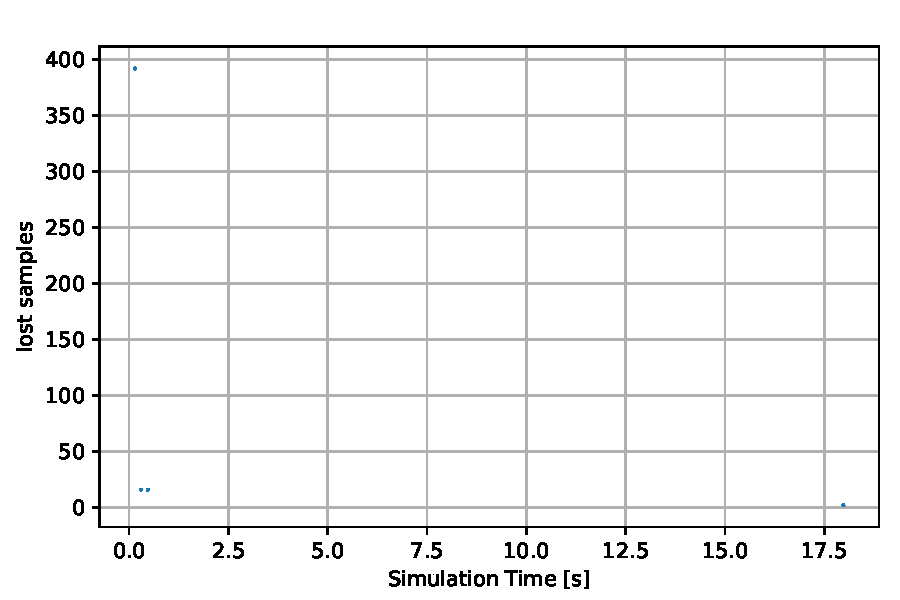
\includegraphics{graficas/RED/muestras_perdidas_red.pdf}
    \caption{Muestras perdidas con RED}
    \label{fig:sinqos_pktreceived99100}
\end{figure}




 %%%%%%%%%%%%%%%%%%%%%%%%%%%%%%%%%%%%%%%%
 % Apéndices, glosarios e bibliografía  %
 %%%%%%%%%%%%%%%%%%%%%%%%%%%%%%%%%%%%%%%%

%\appendix
%\appendixpage
%\chapter{Material adicional}
\label{chap:adicional}

\lettrine{E}{xemplo} de capítulo con formato de apéndice, onde se pode
incluír material adicional que non teña cabida no corpo principal do
documento, suxeito á limitación de 80 páxinas establecida no
regulamento de TFGs.

\Blindtext

%\include{anexos/...}

%\printglossary[type=\acronymtype,title=\nomeglosarioacronimos]
%\printglossary[title=\nomeglosariotermos]

%\bibliographystyle{IEEEtranN}
%\bibliography{\bibconfig,bibliografia/bibliografia}
%\clearpage
 
\end{document}

%%%%%%%%%%%%%%%%%%%%%%%%%%%%%%%%%%%%%%%%%%%%%%%%%%%%%%%%%%%%%%%%%%%%%%%%%%%%%%%%
